\documentclass[12pt]{article}
\usepackage[paper=letterpaper,margin=1.5cm]{geometry}
\usepackage{amsmath}
\usepackage{amssymb}
\usepackage{amsfonts}
\usepackage{mathtools}
%\usepackage[utf8]{inputenc}
%\usepackage{newtxtext, newtxmath}
\usepackage{lmodern}     % set math font to Latin modern math
\usepackage[T1]{fontenc}
\renewcommand\rmdefault{ptm}
%\usepackage{enumitem}
\usepackage[shortlabels]{enumitem}
\usepackage{titling}
\usepackage{graphicx}
\usepackage[colorlinks=true]{hyperref}
\usepackage{setspace}
\usepackage{subfigure} 
\usepackage{braket}
\usepackage{color}
\usepackage{tabularx}
\usepackage[table]{xcolor}
\usepackage{listings}
\usepackage{mathrsfs}
\usepackage{stackengine}
\usepackage{physics}
\usepackage{afterpage}
\usepackage{pdfpages}
\usepackage[export]{adjustbox}
\usepackage{biblatex}

\setstackEOL{\\}

\definecolor{dkgreen}{rgb}{0,0.6,0}
\definecolor{gray}{rgb}{0.5,0.5,0.5}
\definecolor{mauve}{rgb}{0.58,0,0.82}


\lstset{frame=tb,
  language=Python,
  aboveskip=3mm,
  belowskip=3mm,
  showstringspaces=false,
  columns=flexible,
  basicstyle={\small\ttfamily},
  numbers=none,
  numberstyle=\tiny\color{gray},
  keywordstyle=\color{blue},
  commentstyle=\color{dkgreen},
  stringstyle=\color{mauve},
  breaklines=true,
  breakatwhitespace=true,
  tabsize=3
}
\setlength{\droptitle}{-6em}

\makeatletter
% we use \prefix@<level> only if it is defined
\renewcommand{\@seccntformat}[1]{%
  \ifcsname prefix@#1\endcsname
    \csname prefix@#1\endcsname
  \else
    \csname the#1\endcsname\quad
  \fi}
% define \prefix@section
\newcommand\prefix@section{}
\newcommand{\prefix@subsection}{}
\newcommand{\prefix@subsubsection}{}
\renewcommand{\thesubsection}{\arabic{subsection}}
\makeatother
\DeclareMathOperator*{\argmin}{argmin}
\newcommand{\partbreak}{\begin{center}\rule{17.5cm}{2pt}\end{center}}
\newcommand{\alignbreak}{\begin{center}\rule{15cm}{1pt}\end{center}}
\newcommand{\tightalignbreak}{\vspace{-5mm}\alignbreak\vspace{-5mm}}
\newcommand{\hop}{\vspace{1mm}}
\newcommand{\jump}{\vspace{5mm}}
\newcommand{\R}{\mathbb{R}}
\newcommand{\C}{\mathbb{C}}
\newcommand{\N}{\mathbb{N}}
\newcommand{\G}{\mathbb{G}}
\renewcommand{\S}{\mathbb{S}}
\newcommand{\bt}{\textbf}
\newcommand{\xdot}{\dot{x}}
\renewcommand{\star}{^{*}}
\newcommand{\ydot}{\dot{y}}
\newcommand{\lm}{\mathrm{\lambda}}
\renewcommand{\th}{\theta}
\newcommand{\id}{\mathbb{I}}
\newcommand{\si}{\Sigma}
\newcommand{\Si}{\si}
\newcommand{\inv}{^{-1}}
\newcommand{\T}{^\intercal}
\renewcommand{\tr}{\text{tr}}
\newcommand{\ep}{\varepsilon}
\newcommand{\ph}{\varphi}
%\renewcomand{\norm}[1]{\left\lVert#1\right\rVert}
\definecolor{cit}{rgb}{0.05,0.2,0.45}
\addtolength{\jot}{1em}
\newcommand{\solution}[1]{

\noindent{\color{cit}\textbf{Solution:} #1}}

\newcounter{tmpctr}
\newcommand\fancyRoman[1]{%
  \setcounter{tmpctr}{#1}%
  \setbox0=\hbox{\kern0.3pt\textsf{\Roman{tmpctr}}}%
  \setstackgap{S}{-.9pt}%
  \Shortstack{\rule{\dimexpr\wd0+.1ex}{.9pt}\\\copy0\\
              \rule{\dimexpr\wd0+.1ex}{.9pt}}%
}

\newcommand{\Id}{\fancyRoman{2}}

% Enter the specific assignment number and topic of that assignment below, and replace "Your Name" with your actual name.
\title{STAT 31210: Homework 2}
\author{Caleb Derrickson}
\date{January 19, 2024}

\begin{document}
\onehalfspacing
\maketitle
\allowdisplaybreaks
{\color{cit}\vspace{2mm}\noindent\textbf{Collaborators:}} The TA's of the class, as well as Kevin Hefner, and Alexander Cram.

\tableofcontents

\newpage
\section{Problem 2.3}
Suppose that $f: G\rightarrow \R$ is a uniformly continuous function defined on an open subset $G$ of a metric space $X$. Prove that $f$ has a unique extension to a continuous function $\overline{f} : \Bar{G} \rightarrow \R$ defined on the closure $\Bar{G}$ of $G$. Show that such an extension need not exist if $f$ is continuous but not uniformly continuous on $G$.

\newcommand{\fbar}{\Bar{f}}

\partbreak
\begin{solution}

    Suppose we have a sequence $x_n \in \Bar{G}$. Since $\Bar{G}$ is closed, we can assume this sequence converges to the value $x \in \Bar{G}$. Define the extension $\fbar : \Bar{G} \rightarrow \R$ as $\fbar (x) = \lim_{n \rightarrow \infty} f(x_n)$. Note for all $n \in \N, x_n \in G$. And since $f$ is uniformly continuous on $G$, and also $x_n$ is Cauchy (it converges), $f(x_n)$ is then Cauchy. This is because for any sufficiently large $n, m \in \N$, we can make $d(x_n, x_m)$ arbitrarily small, i.e. less than some $\ep > 0$. $f$ is uniformly continuous, so for points close enough in the domain (take $x, y$), then their distance in the target space is also arbitrarily small. Therefore, for sufficiently large $N \in \N$ and $n, m \geq N$, we see that $d(x_n, x_m) < \ep$ for any $\ep > 0$. Therefore, $d(f(x_n), f(x_m)) < \ep$. \par

    \jump
    Note that the target space, $\R$, is complete, so stating $\fbar(x \in \Bar{G}) = \lim_{n\rightarrow \infty} f(x_n)$ is well defined. We need to show now that $\fbar$ is unique and uniformly continuous. 

    \tightalignbreak
    \begin{itemize}[-]
        \item \underline{$\fbar$ is unique.}

        \jump
        Since $\R$ is complete and $f(x_n)$ is Cauchy, then the sequence has a limit, so this is well defined. If $a, b \in \R$, and $a = \lim_{n \rightarrow \infty} \fbar(x_n) = b$, then by the triangle inequality, 
        \[d(a, b) \leq d(a, f(x_n)) + d(f(x_n), b).\]
        Since $f(x_n) \rightarrow a$ and $f(x_n) \rightarrow b$, these two distances will approach zero in the limit as $\ep \rightarrow 0$. Therefore, $d(a, b) \leq \ep \rightarrow 0$, so $d(a, b) = 0 \iff a = b$. Therefore, $\fbar$ is unique.

        \item \underline{$\fbar$ is uniformly continuous.}

        \jump
        Since $f$ is continuous, there exists a $\delta > 0$ such that for $d(x, y) < \delta / 3, \ d(f(x), f(y)) < \ep / 3$, for some $\ep > 0$, and for any $x, y \in \Bar{G}$. Since $\Bar{G}$ is closed, there exists sequences $x_n \in G, \ y_n \in G$ for which $x_n \rightarrow x$ and $y_n \rightarrow y$ as $n \rightarrow \infty$. Explicitly, we see when $n \geq N_1 \in \N$, we can have $d(x_n, x) < \delta / 3$ and $d(y_n, y) < \delta / 3$. \par

        \jump
        When $n \geq N_1$, we see $d(x_n, y_n) \leq d(x_n, x) + d(x, y) + d(y, y_n)$ by the triangle inequality. These can all be made less than $\delta / 3$, therefore $d(x_n, y_n) < \delta$. This will imply that their distances under the transformation can be made arbitrarily small. In this case, we let $d(f(x_n), f(y_n)) < \ep / 3$. \par

        \jump
        Since $f(x_n)$ and $f(y_n)$ are both Cauchy sequences in $\R$, we see that $f(x_n) \rightarrow \fbar(x)$ and $f(y_n) \rightarrow \fbar(y)$. Therefore, there exists an $\N_2 \in \N$ such that, when $n \geq N_2$, implies both $d(f(x_n), \fbar(x))$ and $d(f(y_n), \fbar(y)$ can be made less than $\delta / 3$. Choose $N = \max \{ N_1, N_2 \}$. Therefore, for any $n \geq N$, 
        \[d(\fbar(x), \fbar(y)) \leq d(\fbar(x), f(x_n)) + d(f(x_n), f(y_n)) + d(f(y_n), \fbar(y)).\]
        All terms on the right hand side were shown to be less than $\ep / 3$. Therefore, $d(\fbar(x), \fbar(y)) < \ep$, implying $\fbar$ is uniformly continuous.
    \end{itemize}
\end{solution}

\newpage
\section{Problem 2.6}
Show that the space $C([a, b])$ equipped with the $L^1$-norm $\norm{\cdot}_1$ defined as 
\[\norm{f}_1 = \int_a^b |f(x)| \ dx\]
is incomplete. Show that if $f_n \rightarrow f$ with respect to the sup-norm, then $f_n \rightarrow f$ with respect to $\norm{\cdot}_1$. Give a counterexample to show the converse is not true.
\partbreak
\begin{solution}

    \begin{itemize}[-]
        \item \underline{Incompleteness with respect to $\norm{\cdot}_1$.}

        \jump
        For $n \in \N$, consider the sequence of functions:
        \[
        f_n(x) = \begin{cases}
            1, & x \in [a, \frac{b - a}{2}]\\
            1 - \frac{n}{b - a}(x - \frac{b - a}{2}), &x \in (\frac{b - a}{2},  \frac{b - a}{2} + \frac{b - a}{n}]\\
            0, & x \in (\frac{b - a}{2} + \frac{b - a}{n}, b]
        \end{cases}
        \]
        This sequence of funcitons converges to the step function, where we ``step down" from 1 to zero at the midpoint $\frac{b -a}{2}$. Figure \ref{fig:p2.6.1} shows the function sequence for the first few $n$ values, as well as $\norm{f_n - f}_1$, where $f$ is the sequence limit. More explicitly, we can evaluate the difference integral as 
        \[
        \int_a^b |f_n(x) - f(x)| \ dx = \int_{\frac{b - a}{2}}^{\frac{b - a}{2} + \frac{b - a}{n}} 1 - \frac{n}{b - a} \Big(x - \frac{b - a}{2}\Big) \ dx = \frac{b - a}{2n} \rightarrow 0 \text{ as } n \rightarrow \infty. 
        \]
        It's easy to see that $f_n$ is a cauchy sequence of continuous functions over $[a, b]$. However, since the limit $f$ is not continuous, $C([a, b])$ is incomplete with respect to $\norm{\cdot}_1$. 
        

        \begin{figure}[!h]
            \centering
            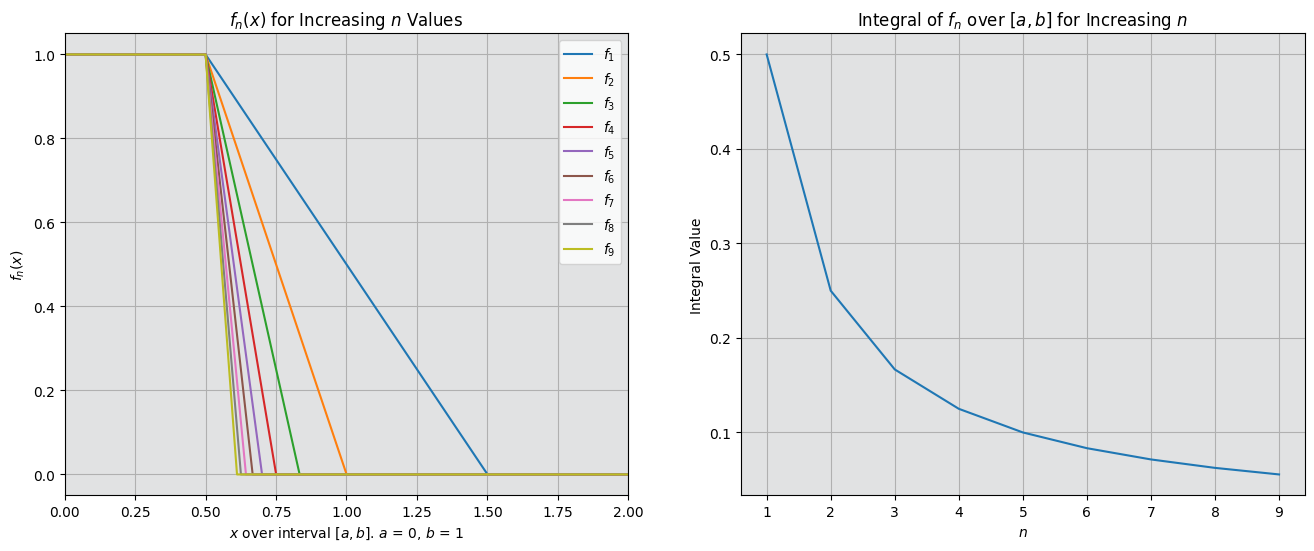
\includegraphics[width = 0.6\textwidth]{Images/Problem2.6.1.png}
            \caption{(Left) The sequence of functions $f_n$ described in Problem 2.6. The sequence ``steps down" from 1 to zero at the midpoint. (Right) The value of $\norm{f_n - f}_1$, where $\norm{\cdot}_1$ is the $L^1$ norm.}
            \label{fig:p2.6.1}
        \end{figure}

        \clearpage
        \item \underline{Convergence wrt sup-norm implies convergence wrt $\norm{\cdot}_1$.}

        \jump
        Let $[a, b] = I$. We are given that $f_n \rightarrow f$ as $n \rightarrow \infty$ with respect to the sup norm. Thus, there exists $N \in \N$ such that when $n \geq N$ implies $\sup_{x \in I} |f_n(x) - f(x)| < \ep / (b - a)$. Thus, for any $x \in I$, $|f_n(x) - f(x)| < \ep / (b - a)$. Integrating both sides over $I$ yields
        \[\int_I |f_n(x) - f(x)| \ dx < \int_I \frac{\ep}{(b - a)} \ dx = \ep. \]
        The above inequality gives us $\norm{f_n(x) - f(x)}_1 \rightarrow 0$ as $n \rightarrow \infty$. 

        \item \underline{Counterexample of the converse.}
        
        Taking my example from part, 1, we can see that $f_n$ converges to zero with respect to $\norm{\cdot}_1$, but under the sup-norm, $|f_n(x) - f(x)| = 1$ for all finite $n$. This will not converge to zero in the sup norm, providing a sufficient counterexample.
    \end{itemize}
\end{solution}
\clearpage

\newpage
\section{Problem 2.9}
Let $w : [0, 1] \rightarrow \R$ be a nonnegative, continuous function. For $f \in C([0, 1])$, define the weighted supremum norm by $\norm{f}_w = \sup_{0 \leq x \leq 1} \{ w(x)|f(x)|\}$.
\subsection{Problem 2.9, part 1}
If $w(x) > 0$ for $0 < x < 1$, show that $\norm{\cdot}_w$ is a norm on $C([0, 1])$.
\partbreak
\begin{solution}

    We just need to show the conditions for a norm hold. I will suppress the supremum bounds for legibility.
    \tightalignbreak
    \begin{itemize}[-]
        \item \underline{Absolute homogeneity.}

        \jump
        Suppose $\lm \in \R, f \in C([0, 1])$. Then, 
        \[\norm{\lambda f}_w = \sup \{ w(x)|\lm f(x)| \} = \sup \{ w(x)|\lm| |f(x)| \} = |\lm|\sup \{ w(x)|f(x)| \} = |\lm| \norm{f}_w\]

        \item \underline{Positive definiteness.}

        \jump
        If $\norm{f}_w = 0$, then $w(x)|f(x)| = 0$ for all $x \in [0, 1]$. Since $w(x) > 0$ for $0 < x < 1$, we can conclude $|f(x)| = 0$ for $x \in (0, 1)$. This can be extended to $[0, 1]$ since $f$ is continuous, so $f(0)$ and $f(1)$ cannot hold any nonzero value. Therefore, $f = 0$.  \par

        \jump
        If $f = 0$, then $\norm{f}_w = \sup \{ w(x) \cdot 0 \} = 0$ for all $x \in [0, 1]$. Therefore, $\norm{f}_1 = 0$. 

        \item \underline{Triangle Inequality.}

        \jump
        If $f, g \in C([0, 1])$, Then by the triangle inequality over $\R$,
        \begin{align*}
            \norm{f + g}_w &= \sup \{ w(x)|f(x) + g(x)| \} \leq \sup \{ w(x) (|f(x) + g(x)|)\} \\
            &\leq \sup \{w(x)|f(x)|\} + \sup\{w(x)|g(x)|\}\\ 
            &= \norm{f}_w + \norm{g}_w \\ 
            \implies \norm{f + g}_w &\leq \norm{f}_w + \norm{g}_w
        \end{align*}
    \end{itemize}
\end{solution}

\newpage
\subsection{Problem 2.9, part 2}
If $w(x) > 0$ for $x \in [0, 1]$, show that $\norm{\cdot}_w$ is equivalent to the usual sup-norm, corresponding to $w = 1$.
\partbreak
\begin{solution}

    By the definition in Chapter 5, we wish to ind a $c_1, c_2 > 0$ for which
    \[c_1\norm{f}_\infty \leq \norm{f}_w \leq c_2\norm{f}_\infty. \]
    Notice that 
    \[\norm{f}_w = \sup \{w(x)|f(x)|\} \leq \sup\{w(x)\}\sup\{|f(x)|\} = \sup\{w(x)\}\norm{f}_\infty\]
    So take $c_2 = \sup \{w(x)\}$. Next, consider $\inf\{w(x)\}$. Note that, since $w$ is a continuous function over a closed interval, then $w$ attains it maximum and minimum. Since $w(x) > 0$ for $x \in[0, 1]$, then $\min \{w(x)\} > 0$. Notice then, by the definition of minimum, 
    \[\inf\{w(x)\}\norm{f}_\infty = \sup\{\inf\{w(x)\}|f(x)|\} \leq \sup\{w(x)|f(x)|\} = \norm{f}_w\]
    So then take $c_1 = \min\{w(x)\}$. We have thus found $c_1, c_2$ for which the chain of inequalities is satisfied.    
\end{solution}

\newpage
\subsection{Problem 2.9, part 3}
Show that the norm $\norm{\cdot}_x$ corresponding to $w(x) = x$ is not equivalent to the usual sup-norm.
\partbreak
\begin{solution}

    From the argument I made in the previous part, since $w(0) = 0$, then $\min\{w(x): x \in [0, 1]\} = 0$. This then causes issues when passing into the supremum, so a similar argument cannot be made. Note that this equivalence should hold for all $f \in C([0, 1])$, so an example showing equivalence is broken is sufficient. In the spirit of the example from the previous problem, take
    \[f_n(x) = \begin{cases}
        1 - nx, &x \in [0, 1/n],\\
        0,      &x \in (1/n, 1].
    \end{cases}\]
    We note that $f_n(x)$ is piece-wise continuous for any $n \in \N$. Furthermore, $\norm{f_n}_\infty = 1$. However, under the weighted supremum norm,
\[\norm{f_n}_x = \underset{x \in [0, 1/n]}{\text{sup}} \big\{ x(1 - nx)\big\} = \underset{x \in [0, 1/n]}{\text{sup}} \big\{x - nx^2\big\} = \frac{1}{4n}\footnote{This was calculated using simple maxima rules of Calculus.} \rightarrow 0 \text{ as } n \rightarrow \infty.\]
We require there existing $c_2 > 0$ for which $\norm{f}_\infty \leq c_2 \norm{f}_x$, but it can be shown that as $n \rightarrow \infty$, such a $c_2$ cannot be found. Thus, $\norm{\cdot}_x$ is not equivalent to the usual sup-norm. 
\end{solution}

\newpage
\subsection{Problem 2.9, part 4}
Is the space $C([0, 1])$ equipped with the weighted norm $\norm{\cdot}_x$ a Banach space?
\partbreak
\begin{solution}

    Again, take the example function from the last part. We see that $f_n$ is cauchy under $\norm{\cdot}_x$, since for $m, n$ sufficiently large,
    \[\norm{f_n - f_m}_x = \sup\big \{ x|1 - nx| \big \} = \sup\big \{ x - nx^2 \big \} = \frac{1}{4n}.\]
    Without loss of generality, we assume $m > n$. So that for $x \in [0, 1/n]$, the difference will be maximized for $x \in (1/m, 1/n]$. This would imply $f_m = 0$, therefore will be discarded. This can be made arbitrarily small as $n, m \geq N$ for $N \in \N$, therefore justifying the claim. However, we see the limit, 
    \[
    f(x) = \begin{cases}
        1, &x = 0\\
        0, & x \in (0, 1]
    \end{cases}
    \]
    is not continuous. Therefore, we have found a Cauchy sequence in $C([0, 1])$ which does not have a continuous limit under the weighted norm. Thus $C([0, 1])$ equipped with the weighted norm $\norm{\cdot}_x$ is not a Banach Space. 
\end{solution}
\newpage
\subsection{Problem 2.13}
Consider the scalar initial value problem $\Dot{u}(t) = |u(t)|^\alpha, \ u(0) = 0$. Show that the solution is unique if $\alpha \geq 1$, but not if $0 \leq \alpha < 1$. 
\partbreak
\begin{solution}

    Here we will be invoking the only test for uniqueness for ordinary differential equations found up until this part of the book, which is Theorem 2.26, which for clarity, I will give below. 
    
    \tightalignbreak
    \begin{quote}
        Suppose that $f(t, u)$ is continuous in the rectangle 
        \[R = \{(t, u) : |t - t_0| \leq T, \ |u - u_0| \leq L \}, \]
        and that 
        \[|f(t, u)| \leq M \quad \text{ if } (t, u) \in R.\]
        Let $\delta = \min (T, L / M)$. If $u(t)$ is any solution of the initial value problem, then
        \[|u(t) - u(t_0)| \leq L \quad \text{ when } |t - t_0| \leq \delta.\]
        Suppose, in addition, that $f$ is a Lipschitz continuous function of $u$, uniformly in $t$. Then the solution is unique in the interval $|t - t_0| \leq \delta$.  
    \end{quote}
    \vspace{-6mm}{\alignbreak}

    Since $t_0 = 0$ and $u(t_0) = 0$, the rectangle $R = \{(t, u) : |t| \leq T, \ |u| \leq L \}$. Note that $f = |u|^\alpha$ is continuous for $\alpha \geq 0$. Therefore, by the Mean Value Theorem, there exists $\xi \in (u, v) \subset \R$ for $u, v \in \R$ such that 
    \[f(u) - f(v) = f'(\xi)(u - v),\]
    where
    \[f'(\xi) = \Bigg[\alpha |x|^{(\alpha - 1)} \frac{x}{|x|} \Bigg]\Bigg| _{x = \xi} \leq \frac{\alpha}{|\xi|^{(1 - \alpha)}}\]
    Therefore,
    \[|f(u) - f(v)| \leq \frac{\alpha}{|\xi|^{(1 - \alpha)}}|u - v|, \quad \text{ for } u, v \in R.\]
    Note that it is possible for $\xi = 0$, so the coefficient could be undefined. This inequality is guaranteed only when $\alpha \geq 1$ ($0 \leq \alpha < 1$ allows for undefined behavior). Therefore, $f$ is Lipschitz for $\alpha \geq 1$, and not for $0 \leq \alpha < 1$. Thus, by the theorem above, we have that the initial value problem has a unique solution for $\alpha \geq 1$. Since $f$ is not Lipschitz for $0\leq \alpha < 1$, then the initial value problem is not guaranteed unique solutions.     
\end{solution}

\newpage
\section{Problem 3.5}
An $n \times n$ matrix $A$ is said to be \textit{diagonally dominant} if for each row the sum of the absolute values of the off-diagonal terms is less than the absolute value of the diagonal term. We write $A = D - L - U$ where $D$ is the diagonal, $L$ is lower triangular, and $U$ is upper triangular. If $A$ is diagonally dominant, show that 
\[\norm{L + U}_\infty < \norm{D}_\infty.\]
Use the contraction mapping theorem to prove that if $A$ is diagonally dominant, then $A$ is invertible and that the following iteration schemes converge to a solution of the equation $Ax = b$:
\begin{align}
    &x_{n+1} = D\inv (L + U)x_n + D\inv b,\\
    &x_{n+1} = (D - L)\inv Ux_n + (D - L)\inv b.
\end{align}
What can you say about the rate of convergence?
\partbreak
\begin{solution}

    We will break this problem into sections.
    \begin{itemize}[-]
        \item \underline{$\norm{L + U}_\infty < \norm{D}_\infty.$}

        \jump
        \tightalignbreak
        \begin{align*}
            |a_{ii}| &> \sum_{j \neq i} |a_{ij}| &\text{(Given for all $ i \leq n$.)}\\
            |a_{ii}| &> \sum_{j < i} |a_{ij}| + \sum_{j > i} |a_{ij}| &\text{(Breaking up sum.)}\\
            \implies &\underset{i \leq n}{\max} \left\{ |a_{ii}| \right\} > \underset{i \leq n}{\max} \left \{ \sum_{j < i} |a_{ij}| + \sum_{j > i} |a_{ij}| \right\} &\text{(Taking max.)}\\
            \iff & \norm{D}_\infty > \norm{L + U}_{\infty} &\text{(By definitions given.)}
        \end{align*}
        \vspace{-6mm}\alignbreak

        \newpage
        \item \underline{Strict diagonally dominant matrices are invertible.}\footnote{This does not rely on the contraction mapping theorem, it is just a property of strictly diagonally dominant matrices.}

        \jump
        We will show that $Au = 0$ happens only for $u = 0$. Suppose this statement were false, and that $Au = 0$ for $u_i \neq 0$ for any $i \leq n$. Suppose that for $k \leq n, u_k \geq u_i$, that is $u_k$ is the largest element of $u$. Then,
        \[ (Au)_k = \sum_{j \leq n} a_{kj}u_j = 0 \implies  a_{kk}u_k = -\sum_{j \neq k} a_{kj}u_j.\]
        Taking absolute values gives the following:
        \tightalignbreak
        \begin{align*}
        |a_{kk}u_k| &= \Big| \sum_{j \neq k} a_{kj}u_j\Big| &\text{(Taking absolute values.)}\\
        &\leq \sum_{j \neq k}\left| a_{kj} u_j\right| &\text{(Triangle inequality.)}\\
        &= \sum_{j \neq k}\left| a_{kj} \right| \left|u_j\right| &\text{(Over $\R$.)}\\
        \implies & |a_{kk}| \leq \frac{1}{|u_k|}\sum_{j \neq k}\left| a_{kj} \right| \left|u_j\right| &\text{(Rearranging.)}\\
        \implies & |a_{kk}| \leq \sum_{j \neq k}\left| a_{kj} \right| \left|\frac{u_j}{u_k}\right| &\text{(Rearranging.)}\\
        \implies & |a_{kk}| \leq \sum_{j \neq k}\left| a_{kj} \right| &\text{($u_k$ is max element of $u$.)}
        \end{align*}
        \vspace{-6mm}\alignbreak
        
        We know that $A$ is strictly diagonally dominant, which means $|a_{ii}| > \sum_{i \neq j} |a_{ij}|$ for any $i \leq n$. We found the contrary, however, which is a contradiction. Therefore, $u = 0$. So $A$ is invertible.

        \newpage
        \item \underline{Convergence of Schemes.}

        \jump
        Consider the iteration $x_{n+1} = D\inv (L + U)x_n + D\inv b$ and take $T(x) = D\inv (L + U)x + D\inv b$.\footnote{In general, $T(x) \in \R^n$. For now, just assume the absolute value is the infinity norm.} We want to show that $T$ is a contraction map. Since $T$ is linear, we can say
        \[|T(x) - T(y)| = |D\inv (L + U)(x - y)| \leq \norm{D\inv (L + U)}_\infty |x - y|.\]
        We just need to show that $\norm{D\inv (L + U)}_\infty < 1$. Since $A$ is strictly diagonally dominant, we can see that
        \[\norm{D\inv (L + U)}_\infty = \underset{i \leq n}{\max} \bigg\{ \frac{1}{|a_{ii}|}\sum_{j \leq n} |a_{ij}| \bigg\} < 1\]
        Therefore, $T$ is a contraction mapping. By the contraction mapping theorem, there is a fixed point of the mapping $x$, such that $T(x) = x$. So
        \[D\inv (L + U)x + D\inv b = x \implies (L+U)x + b = Dx \implies b = (D - L - U)x \implies Ax = b.\]
        Next consider the mapping $T(x) = (D - L)\inv Ux + (D - L)\inv b$. We need to first show it is a contraction mapping. Following the same logic as above, we need to show $\norm{(D - L)\inv U}_\infty < 1$. Suppose that $x$ is an eigenvector of $(D - L)\inv U$ with eigenvalue $\lm$. We need to show that $|\lm| < 1$. That is, 
        \tightalignbreak
        \begin{align*}
            (D - L)\inv Ux &= \lm x &\text{(Given.)}\\
            \lm (D - L)x &= Ux &\text{(Inverting.)}\\
            \lm \Big ( \sum_{j \geq i} a_{ij} x_j\Big ) &= -\sum_{j < i} a_{ij}x_j &\text{(For all $i \leq n$.\footnote{$i$ and $j$ might be flipped in the summation indices, but this doesn't change the result.})}\\
            \lm a_{ii}x_i &= -\Big( \sum_{j > i} a_{ij}x_j + \lm \sum_{j < i}a_{ij}x_j \Big) &\text{(Rearranging.)}\\
            |\lm a_{ii}x_i| &= \Big| \sum_{j > i} a_{ij}x_j + \lm \sum_{j < i}a_{ij}x_j \Big| &\text{(Taking absolute vales.)}\\
            |\lm a_{ii}x_i| &\leq \Big| \sum_{j > i} a_{ij}x_j\Big| + \Big|\lm \sum_{j < i}a_{ij}x_j \Big| &\text{(Triangle Inequality.)}\\
            |a_{ii}| &\leq \frac{1}{|\lm x_i|} \Big| \sum_{j > i} a_{ij}x_j\Big| + \Big|\lm \sum_{j < i}a_{ij}x_j \Big| &\text{(Rearranging.)}\\
            |a_{ii}| &\leq \frac{1}{|\lm x_i|} \Big( \sum_{j > i} |a_{ij}||x_j| + |\lm| \sum_{j < i}|a_{ij}||x_j| \Big) &\text{(Cauchy Schwartz.)}\\
            |a_{ii}| &\leq \frac{1}{|\lm|} \sum_{j > i} |a_{ij}|\frac{|x_j|}{|x_i|} + \sum_{j < i}|a_{ij}|\frac{|x_j|}{|x_i|} &\text{(Rearranging.)}\\
            |a_{ii}| &\leq \frac{1}{|\lm|} \sum_{j > i} |a_{ij}| +  \sum_{j < i}|a_{ij}| &(|x_i| \geq |x_j|.\footnote{\text{Assume without loss of generality this is true.}})\\
            |a_{ii}| &\leq \frac{1}{|\lm|} \sum_{j > i} |a_{ij}| + \sum_{j < i}|a_{ij}| + \Big( \sum_{j > i}|a_{ij}| - \sum_{j > i}|a_{ij}|\Big) &\text{(Adding a zero.)}\\
            |a_{ii}| &\leq \bigg(\frac{1}{|\lm|} - 1 \bigg) \sum_{j > i} |a_{ij}| + \sum_{j < i}|a_{ij}| + \sum_{j > i}|a_{ij}| &\text{(Rearranging.)}\\
            |a_{ii}| &< \bigg(\frac{1}{|\lm|} - 1 \bigg) \sum_{j > i} |a_{ij}| + |a_{ii}| &\text{(A is strictly diagonal dominant.)}\\
            0 &< \bigg(\frac{1}{|\lm|} - 1 \bigg) \sum_{j > i} |a_{ij}| &\text{(Simplifying.)}\\
            \implies 0 &< \bigg(\frac{1}{|\lm|} - 1 \bigg) &\text{(Sum cannot be negative.)}\\
            \implies 1 &> |\lm| &\text{(Rarranging and Taking Reciprocal.)}
        \end{align*}
        \vspace{-6mm}\alignbreak
        Thus, we have shown that all eigenvalues of $(D - L)\inv U$ have magnitude less than 1\footnote{The case where $\lm = 0$ implies that $x \in \ker U$. Let's assume this is not the case.}, so $T$ is then a contraction mapping. Therefore by the Contraction Mapping theorem, there exists a fixed point $x$ of the mapping such that $Tx = x$. This then implies the following chain: 
        \[(D - L)\inv Ux + (D - L)\inv b = x \implies Ux + b = (D - L)x \implies (D - L - U)x = b \implies Ax = b.\]

        \item \underline{Rate of Convergence.}
        
        Since the two sequences converge, we can at least say they converge linearly. Furthermore, the two sequences are known only to converge when the matrix A is either strictly diagonally dominant, symmetric, or positive definite. In order to determine the rate of convergence, we would need to determine the ratio
        \[\frac{\norm{x_{n+1} - x^*}}{\norm{x_n - x^*}}, \quad x^* = A\inv b.\]
        It is likely the case that you can directly prove that this ratio is less than 1, since both matrices acting on the prior sequence have their max eigenvalue less than 1. This leads to some tricky algebra, which I wasn't successful in showing. 
    \end{itemize}
\end{solution}

\newpage
\section{Problem 3.6}
The following integral equation for $f: [-a, a] \rightarrow \R$ arises in a model of the motion of gas particles on a line:
\[f(x) = 1 + \frac{1}{\pi} \int_{-a}^a \frac{1}{1 + (x - y)^2}f(y)dy \quad \text{(for $-a \leq x \leq a.$)}\]
Prove that this equation has a unique bounded continuous solution for every $0 < a < \infty$. Prove that the solution is nonnegative. What can you say if $a = \infty$?
\partbreak
\begin{solution}

    By theorem 3.3, we first need to show that $T$ defined as the integral above is a contraction mapping. Take any continuous functions $f_1, f_2: [-a, a] \rightarrow \R$.
    \tightalignbreak
    \begin{align*}
        \norm{T(f_1) - T(f_2)}_\infty &= \frac{1}{\pi}\norm{\int_{-a}^a \frac{f_1(y) - f_2(y)}{1 + (x - y)^2}\ dy}_\infty &\text{(To Show.)}\\
        &= \frac{1}{\pi}\sup_{x \in [-a, a]} \Bigg|\int_{-a}^a \frac{f_1(y) - f_2(y)}{1 + (x - y)^2}\ dy \Bigg| &\text{(Definition of $\norm{\cdot}_\infty$}\\
        &\leq \frac{1}{\pi}\sup_{x \in [-a, a]} \int_{-a}^a \frac{|f_1(y) - f_2(y)|}{1 + (x - y)^2}\ dy &\text{(Triangle Inequality.)}\\
        &\leq \frac{1}{\pi} \norm{f_1 - f_1}_\infty \sup_{x \in [-a, a]}\int_{-a}^a \frac{1}{1 + (x - y)^2} \ dy &\text{(Cauchy Schwartz.)}\\
        & = \frac{1}{\pi}\norm{f_1 - f_1}_\infty \sup_{x \in [-a, a]} \big\{ \arctan(x + a) - \arctan(x - a)\big\} &\text{(Solving integral.)}\\
        &\leq \frac{1}{\pi}\norm{f_1 - f_2}_\infty\sup_{x \in [-a, a]} \arctan \left( \frac{2a}{1 + x^2 - a^2}\right) &\text{(Trig Identity.)}\\
        &\leq \frac{1}{\pi} \norm{f_1 - f_2}_\infty\left ( \frac{\pi}{2}\right) &\text{(Sup of arctan.)}\\
        \implies \norm{T(f_1) - T(f_2)}_\infty &\leq  \frac{1}{2} \norm{f_1 - f_2}_\infty &\text{(Simplifying.)}
    \end{align*}
    \vspace{-6mm}\alignbreak
    Note that $T: C[-a, a] \rightarrow C[-a, a]$ since the integral operation is a continuous mapping. Therefore, since $T$ is a contraction mapping with $c = 1/2$, by theorem 3.3, $f$ is unique an continuous on the interval. Note also that since the interval is closed, bounded and $f \in C[-a, a]$, $f$ is bounded. \par
    \newpage
    However, if we take $a = \infty$, everything up to applying the bounds on the integral solution holds. When we do apply the bounds, we see
    \[\int_{-\infty}^\infty \frac{1}{1+(x - y)^2} \ dy = \Big[\arctan (x - y) \Big]_{y = -\infty}^{y = \infty} = \pi\]
    Therefore, we see that $ \norm{T(f_1) - T(f_2)}_\infty \leq \norm{f_1 - f_2}_\infty$, which implies $c = 1$. This implies that $T$ is not a strict contraction mapping. Next we want to show that $f$ is nonnegative, which we will prove by contradiction. That is, suppose $f(z) < 0$ for some $z \in [-a, a]$. Suppose further that $f(z) = \min_{x \in [-a, a]} f(x)$. The following statements can then be made:
    \tightalignbreak
    \begin{align*}
        f(z) &= 1 + \frac{1}{\pi}\int_{-a}^a \frac{1}{1 + (z - y)^2} f(y) \ dy &\text{(Given.)}\\
        &\geq 1 + \frac{1}{\pi}\int_{-a}^a \frac{1}{1 + (z - y)^2} f(z) \ dy &\text{($f(z)$ is min.)}\\
        &= 1 + \frac{ f(z)}{\pi} \arctan\left( \frac{2a}{1 + z^2 - a^2} \right) &\text{(Solving integral.)}\\
        &\geq 1 - \frac{f(z)}{2} &(-\frac{\pi}{2} \leq \arctan (x) \leq \frac{\pi}{2}.)\\
        \implies f(z) &\geq 1 - \frac{1}{2}f(z) \\
        f(z) &\geq \frac{2}{3} &\text{(Simplifying.)}
    \end{align*}
    \vspace{-6mm}\alignbreak
    We see then a contradiction, since we require $f(z)$ to be both positive and negative. Therefore, $f$ is a positive function. 
\end{solution}

\newpage


\section{Problem 3.7}
Prove that there exists a unique solution of the following nonlinear BVP when the constant $\lm$ is sufficiently small, 
\begin{gather*}
    -u'' + \lm \sin u = f(x),\\
    u(0) = 0, \quad u(1) = 0.
\end{gather*}
Here, $f: [0, 1] \rightarrow \R$ is a given continuous function. Write out the first few iterates of a uniformly convergent sequence of approximations, beginning with $u_0 = 0$.
\partbreak
\begin{solution}

    We start by multiplying both sides by the Greens function, as used in proposition 3.3 in the text. Note that this is the same form of the operator as described in the book ($A = -d^2 /dx^2 $), so this is justified. Then integrating both sides on the given bounds by $y$ gives
    \[-\int_0^1u''(y)G(x, y) \ dy = \int_0^1 (f(y) - \lm \sin(u(y))) G(x, y) \ dy.\]
    Investigating the left hand side first, we can break this integration up by the case on $y$. In particular,
    \[\int_0^1 y''(y)G(x, y) \ dy = \int_0^x u''(y)(y(1 - x)) \ dy + \int_x^1 u''(y)(x(1 - y)) \ dy.\]
    Via Integration by parts, and noting that $x$ is a constant when differentiating by $y$, this is equivalent to just $u(x)$. Therefore, we have 
    \[\Big[ u'(y)y(1 - x)\Big]_{y = 0}^{y = x} - (1 - x)\int_0^x u'(y) \ dy - \Big[ x(1 - y)u'(y)\Big]_{y = x}^{y = 1} - x\int_x^1 u'(y) \ dy,\]
    \[-(1 - x)\int_0^x u'(y) \ dy - x\int_x^1 u'(y) \ dy\]
    \[ -\int_0^x u'(y) \ dy - x\int_0^1 u'(y) \ dy\]
    \[-u(x)\]
    Reincorporating the right hand side, we get
    \[u(x) = \int_0^1 (f(y) - \lm \sin(u(y))) G(x, y) \ dy.\]
    Define the mapping $T$ as its action on $u$ as shown on the right hand side, i.e.,
    \[T[u](x) = \int_0^1 (f(y) - \lm \sin(u(y)) G(x, y) \ dy.\]
    Note that integration maps continuous functions to continuous functions. Furthermore, $T[u](0) = 0 = T[u](1)$ by the boundary conditions on the problem, as well as the definition of the Green's Function. Therefore, $T: C([0, 1]) \rightarrow C([0, 1])$. We will show this is a contraction mapping when $\lm$ is chosen sufficiently small. For $u, v \in C([0, 1])$,
    \tightalignbreak
    \begin{align*}
        \norm{Tu - Tv}_\infty &= \norm{\int_0^1 \lm \sin(u(y)) G(x, y) \ dy - \int_0^1 \lm \sin(v(y)) G(x, y) \ dy} &\text{(Simplifying.)}\\
        &= |\lm|\norm{\int_0^1 \lm (\sin(u(y)) - \sin(v(y))) G(x, y) \ dy}_\infty &\text{(Norm properties.)}\\
        &\leq |\lm| \int_0^1 \norm{\sin(u) - \sin(v)}_\infty \norm{G(x, y)}_\infty \ dy &\text{(CS and $\triangle$-inequality.)}\\
        &= |\lm| \norm{\sin(u) - \sin(v)}_\infty\int_0^1 \norm{G(x, y)}_\infty \ dy &\text{(Sines are constants.)}\\
        &\leq |\lm| \norm{u - v}_\infty \int_0^1 \norm{G(x, y)}_\infty \ dy &\text{(Sine is Lipschitz with $L = 1$.)}\\
        &\leq |\lm| \norm{u - v}_\infty \sup_{x \in [0, 1]}\int_0^1 |G(x, y)| \ dy &\text{(Norm Definition.)}\\
        &= |\lm| \norm{u - v}_\infty \sup_{x \in [0, 1]}\left[ \int_0^x -y(1 - x) \ dy - \int_x^1 x(1 - y) \ dy \right] &\text{(Greens Function.)}\\
        &= |\lm| \norm{u - v}_\infty \sup_{x \in [0, 1]} \left|\frac{x^2 - x}{2}\right|  &\text{(Evaluating.)}\\
        \norm{Tu - Tv}_\infty&\leq \frac{|\lm|}{8} \norm{u - v}_\infty  &\text{(Check maxima.)}
    \end{align*}
    \vspace{-6mm}\alignbreak
    Therefore, we see that $T$ will only be a contraction when $|\lm| < 8$, satisfying the contraction factor criteria. Since $T$ will be a contraction under that restriction, by the Contraction Mapping Theorem, there will be a fixed point $u$ satisfying $Tu = u$ of the map. We can see that the fixed point is a solution of the system, by taking the second derivative of the mapping. Therefore, the system has a unique solution. Writing the iterates of the mapping is quite tedious, so they will be shorthanded. They will be of the form $u_0 = u,\  u_1 = Tu,\ u_2 = T(T(u)) = T^2(u), \ ..., \ u_k = T^k(u).$ The map $T$ is of the form above.
\end{solution}
\end{document}